\documentclass[10pt]{article}
\usepackage[utf8]{inputenc}
\usepackage{fullpage}
\usepackage{parskip}
\usepackage{amsmath,amssymb,mathtools}
\usepackage{microtype}
\usepackage{booktabs}
\usepackage{graphicx,subfigure}
\usepackage{hyperref} % \url
\usepackage{xcolor} %hilight
\newcommand{\hilight}[1]{\colorbox{yellow}{#1}}
\usepackage{bm}
\newtheorem{theorem}{Theorem}
\usepackage[most]{tcolorbox}
\newtcolorbox[]{solution}[1][]{%
    breakable,
    enhanced,
    colback=white,
    title=Solution,
    #1
}


%% -------------------------------------------
%% Homework-specific macros
%% -------------------------------------------

\usepackage{tikz}
\usetikzlibrary{bayesnet}

\newcommand{\DKL}[2]{D_{\textrm{KL}}\left[#1 \;\|\; #2\right]}
\newcommand{\sbr}[1]{\left[#1\right]}
\newcommand{\rbr}[1]{\left(#1\right)}
\DeclareMathOperator{\E}{\mathbb{E}}
\DeclareMathOperator*{\argmin}{\mathrm{arg\,min}}
\DeclareMathOperator*{\argmax}{\mathrm{arg\,max}}
%% -------------------------------------------

\title{10-708 PGM (Spring 2020): Homework 4}
\author{
\begin{tabular}{rl}
Andrew ID: & [your Andrew ID] \\
Name: & [your first and last name] \\
Collaborators: & [Andrew IDs of all collaborators, if any]
\end{tabular}
}
\date{}

\begin{document}

\maketitle

\section{Variational Autoencoders (Yiwen) [65 pts]}
\label{sec:vae}

\begin{figure}[h]
\centering
\includegraphics[width=0.3\textwidth]{figures/helmholtz-machine.png}
\caption{A \textbf{Helmholtz machine}~\cite{hinton1995wake,dayan2000helmholtz} contains two networks: (1) bottom-up ``recognition'' connections $\phi$ that convert the input data into representations in successive hidden layers, and (2) top-down ``generative'' connections $\theta$ that reconstruct the data from representation in one layer from the representation in the layer above.
\label{fig:helmholtz-machine}}
\end{figure}

The Helmholtz machine (Figure~\ref{fig:helmholtz-machine}) is an architecture that can find hidden structure in data by learning a generative model of the data. Helmholtz machines are usually trained using unsupervised learning algorithms such as the classical \textbf{Wake-Sleep} algorithm~\cite{hinton1995wake} or the modern \textbf{Auto-Encoding Variational Bayes (AEVB)}~\cite{kingma2013auto}, also known as variational autoencoder.

In this problem, you will (re-)derive and implement the Wake-Sleep and AEVB algorithms. The sections are organized as follows:
\begin{itemize}
    \item[(3 pts)] Section~\ref{section:1-elbo}: Derivation of the \textbf{evidence lower bound objective (ELBO)}, which lowerbounds the data log-likelihood $\log p_\theta(\mathbf{x})$.
    \item[(6 pts)] Section~\ref{section:1-Wake-Sleep}: Derivation of the \textbf{Wake-Sleep} algorithm, which alternates between the Wake phase and Sleep phase to optimize an estimate of ELBO.
    \item[(10 pts)] Section~\ref{section:1-aevb}: Derivation of \textbf{AEVB}, which optimizes a stochastic estimate of ELBO.
    \item[(3 pts)] Section~\ref{section:short-questions}: Short-answer questions on Wake-Sleep and AEVB.
    \item[(8 pts)] Section~\ref{section:1-alternate-lower-bound}: Derivation of an \textbf{alternate lower bound} $\mathcal{L}_k(\mathbf{x})$ for the data log-likelihood, which will be used to evaluate trained models in the next section.
    \item[(35 pts)] Section~\ref{section:1-implementation}: Implementations and experiments on the MNIST handwritten digits dataset.
\end{itemize}

{For all parts, assume that latent variables $\mathbf{z}$ are distributed according to a prior $p(\mathbf{z}) = N(0, I)$. The Helmholtz machine tries to learn the \textbf{recognition} parameters $\phi$ and \textbf{generative} parameters $\theta$ such that $$
q_\phi(\mathbf{z} \mid \mathbf{x}) \approx p_\theta(\mathbf{z} \mid x) \propto p_\theta(\mathbf{x}, \mathbf{z})
$$
where:
\begin{itemize}
    \item $q_\phi(\mathbf{z} \mid \mathbf{x})$ is the variational distribution approximating the posterior distribution $p_\theta(\mathbf{z} \mid \mathbf{x})$ for $\mathbf{z}$ given the evidence $\mathbf{x}$. Assume that $q_\phi$ is parameterized by a Gaussian, i.e., $q_\phi(\mathbf{z} \mid \mathbf{x}) = N(\mathbf{z}; \mu_\phi(\mathbf{x}), \Sigma_\phi (\mathbf{x}))$.
    \item $p_\theta(\mathbf{x}, \mathbf{z}) = p(\mathbf{z}) p_\theta(\mathbf{x} \mid \mathbf{z})$ is the joint probability of $(\mathbf{x}, \mathbf{z})$, where $\mathbf{z} \sim p(\mathbf{z})=N(0,I)$, and $\mathbf{x} \sim p_\theta(\mathbf{x} \mid \mathbf{z})$ is the likelihood.
\end{itemize}
} % color{blue}

Assume $\mathbf{x}$ are binary vectors. In other words, $p_{\boldsymbol \theta}(\mathbf{x} \mid \mathbf{z})$ can be modeled with a sigmoid belief net, so the likelihood is of the form $p_\theta(\mathbf{x}|\mathbf{z}) = \text{Bernoulli}( f_\theta (\mathbf{z}) )$. Actually, the data points $\mathbf{x}$ in MNIST take values in $[0, 1]$ rather than $\{ 0, 1\}$, but the loss term $\mathbb{E}_{q}[p_\theta(\mathbf{x} \mid \mathbf{z})]$ still uses sigmoid cross-entropy loss, which is a common practice~\cite{doersch2016tutorial}.

\subsection{Evidence Lower Bound Objective (ELBO)} \label{section:1-elbo}

Suppose we want to learn a directed latent variable model (Figure~\ref{fig:vae}) that is able represent a complex distribution $p(\mathbf{x})$  over the data in the following form:
\begin{equation}
    p_{\boldsymbol \theta}(\mathbf{x}) = \int p_{\boldsymbol \theta}(\mathbf{x} \mid \mathbf{z}) p(\mathbf{z}) d\mathbf{z}
\end{equation}

\begin{figure}[h!]
    \centering
    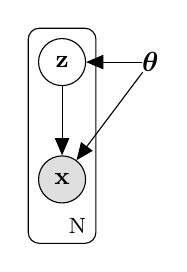
\begin{tikzpicture}
        % Redefine some styles
        \tikzstyle{latent} = [circle,draw=black,inner sep=1pt,
        minimum size=17pt, font=\fontsize{9}{9}\selectfont, node distance=1]

        % Nodes
        \node (x)       [obs]                           {$\mathbf{x}$};
        \node (z)       [latent, above=25pt of x]       {$\mathbf{z}$};
        \node (theta)   [const, right=20pt of z]        {$\boldsymbol \theta$};

        % Plates
        \plate {} {(x)(z)} {N};

        % Edges
        \edge {z}       {x};
        \edge {theta}   {x};
        \edge {theta}   {z};

    \end{tikzpicture}
    \caption{The latent variable model in Problem~\ref{section:1-elbo}.}
    \label{fig:vae}
\end{figure}

Suppose we want to approximate the posterior distribution $p_{\boldsymbol \theta}(\mathbf{z} \mid \mathbf{x})$ using some variational distribution $q_{\boldsymbol \phi}(\mathbf{z} \mid \mathbf{x})$. A tractable way to learn this model is to optimize the \textbf{evidence lower bound objective (ELBO)}, also known as the variational lower bound, defined as follows:
\begin{align*}
\mathcal{L}(\mathbf{x})
&= \mathbb{E}_{\mathbf{z} \sim q_\phi(\mathbf{z} \mid \mathbf{x})} [\log p_\theta(\mathbf{x}, \mathbf{z}) - \log q_\phi(\mathbf{z} \mid \mathbf{x})] \\
&= \int_z q_\phi(\mathbf{z} \mid \mathbf{x}) \log \frac{p_\theta(\mathbf{x}, \mathbf{z})}{q_\phi(\mathbf{z} \mid \mathbf{x})} d \mathbf{z}
\; .
\end{align*}

\begin{itemize}
    \item[(3 pts)] For a single data point $\mathbf{x}^{(i)}$, prove that
    \[
    \log p_\theta(\mathbf{x}^{(i)})
    \geq \mathcal{L}(\mathbf{x}^{(i)}).
    \]
    \begin{solution}
    \end{solution}
\end{itemize}

The above result shows that, for iid data points $\mathbf{x} = \{\mathbf{x}^{(i)}\}_{i=1}^N$,
    \[
    \log p_\theta(\mathbf{x}) \stackrel{\text{iid}}{=} \sum_{i=1}^N \log p_\theta(\mathbf{x}^{(i)})
    \geq \sum_{i=1}^N \mathcal{L}(\mathbf{x}^{(i)})
    = \mathcal{L}(\mathbf{x})
    \]
    which gives the ELBO $\mathcal{L}(\mathbf{x})$ on the data log-likelihood $\log p_\theta(\mathbf{x})$.

\subsection{Wake-Sleep Algorithm}\label{section:1-Wake-Sleep}

In this section, we will derive the optimization objectives for the Wake-Sleep algorithm, which decomposes the optimization procedure into two phases:
\begin{itemize}
\item {\bf Wake}-phase: Given recognition weights $\phi$, we activate the recognition process and update the generative weights $\theta$ to increase the probability that they would reconstruct the correct activity vector in the layer below.
\item {\bf Sleep}-phase: Given generative weights $\theta$, we activate the generative process and update the recognition weights $\phi$ to increase the probability that they would produce the correct activity vector in the layer above. Since it has generated the instance, it knows the true underlying causes, and therefore has available the target values for the hidden units that are required to train the bottom-up weights $\phi$.
\end{itemize}

\subsubsection{Wake-phase}

The Wake-phase fixes the recognition weights $\phi$ and optimizes a Monte Carlo estimate of ELBO w.r.t. the generative weights $\theta$.

\begin{itemize}
    \item[(3 pts)] Given $N$ iid data points $\mathbf{x} = \{\mathbf{x}^{(i)}\}_{i=1}^N$, show that
    \begin{equation}
    \theta^* := {\underset{\theta}{\text{arg max}} } \mathcal{L}(\mathbf{x}) {=
    \underset{\theta}{\text{arg max}} } \sum_{i=1}^N \mathbb{E}_{\mathbf{z} \sim q_\phi(\mathbf{z} \mid \mathbf{x}^{(i)})} \log p_\theta(\mathbf{x}^{(i)} \mid \mathbf{z})
    \label{eq:wake-objective}
    \end{equation}
    which gives the Wake-phase objective.

    \begin{solution}
    \end{solution}
\end{itemize}

\textbf{Wake-phase Pseudocode}: Given $N$ iid data points $\{\mathbf{x}^{(i)}\}_{i=1}^N$, do the following for each $i \in [N]$:
\begin{enumerate}
    \item Feed $\mathbf{x}^{(i)}$ into the recognition network to get $\mu_\phi(\mathbf{x}^{(i)})$ and $\Sigma_\phi(\mathbf{x}^{(i)})$.
    \item  Draw $L$ samples {$\mathbf{z}^{(i)}_1, \ldots, \mathbf{z}^{(i)}_L  \sim q_\phi(\mathbf{z} \mid \mathbf{x}^{(i)}) = N(\mathbf{z}; \mu_\phi(\mathbf{x}^{(i)}), \Sigma_\phi (\mathbf{x}^{(i)}))$ }.
    \item For each $l \in [L]$, feed $\mathbf{z}^{(i)}_l$ into the generative network to get {$f_\theta(\mathbf{z}^{(i)}_l)$ for the likelihood $p_\theta(\mathbf{x} \mid \mathbf{z}^{(i)}_l) = \text{Bernoulli}( \mathbf{x} ; f_\theta( \mathbf{z}^{(i)}_l ))$}.
\end{enumerate}
Finally, use SGD to maximize
\begin{equation}
\max_\theta \sum_{i=1}^N {1 \over L} \sum_{l=1}^L \log p_\theta(\mathbf{x}^{(i)} \mid \mathbf{z}^{(i)}_l)
\end{equation}

This gives a Monte Carlo estimate of the Wake-phase objective in Eq.~\eqref{eq:wake-objective}.

\subsubsection{Sleep-phase}

The Sleep phase fixes the generative weights $\theta$ and updates the recognition weights $\phi$. It is generally intractable to directly minimize the KL-divergence term in $\mathcal{L}(\mathbf{x})$ w.r.t. $\phi$:
    \[
    \argmin_\phi \DKL{ q_{\phi}(\mathbf{z} \mid \mathbf{x}) }{ p_\theta(\mathbf{z} \mid \mathbf{x}) }
    = \argmin_\phi \int_{\mathbf{z}} q_\phi(\mathbf{z} \mid \mathbf{x}) \log { q_\phi(\mathbf{z} \mid \mathbf{x}) \over p_\theta(\mathbf{z} \mid \mathbf{x}) } \; d\mathbf{z}
    \]
    So instead, the Sleep phase minimizes the KL divergence the wrong way round,
    \[
    \argmin_\phi \DKL{ p_\theta(\mathbf{z} \mid \mathbf{x}) }{ q_{\phi}(\mathbf{z} \mid \mathbf{x}) }.
    \]
\begin{itemize}
    \item[(3 pts)] {Suppose we sample $\mathbf{z} \sim p(\mathbf{z}) = N(0, I)$, then sample $\mathbf{x} \sim p_\theta(\mathbf{x} \mid \mathbf{z})$.} Show that
    \begin{equation}
    \phi^* := {\argmin_\phi} \DKL{ p_\theta(\mathbf{z} \mid \mathbf{x}) }{ q_{\phi}(\mathbf{z} \mid \mathbf{x}) }
    {=
    \argmax_\phi} \mathbb{E}_{
    {p_\theta(\mathbf{x}, \mathbf{z})}
    } \sbr{ \log q_\phi(\mathbf{z} \mid \mathbf{x}) }
    \label{eq:sleep-objective}
    \end{equation}
    which gives the Sleep-phase objective.
    \begin{solution}
    \end{solution}
\end{itemize}

\textbf{Sleep-phase Pseudocode}: Let $L \in \mathbb{N}$ be a sample size hyperparameter. For each $l \in [L]$, do the following:
\begin{enumerate}
    \item Draw $\mathbf{z}^l \sim N(0,I)$.
    \item {Sample $\mathbf{x}^l$ from the generative network $p_\theta(\mathbf{x} \mid \mathbf{z}^l) = \text{Bernoulli}(f_\theta(\mathbf{z}^l))$.}
    \item Feed $\mathbf{x}^l$ into the recognition network to get $\mu(\mathbf{x}^l)$ and $\Sigma(\mathbf{x}^l)$.
    \item Compute $q_\phi(\mathbf{z}^l \mid \mathbf{x}^l) = N(\mathbf{z}^l; \mu(\mathbf{x}^l), \Sigma(\mathbf{x}^l))$.
\end{enumerate}

Finally, do SGD to maximize
\begin{equation}
\max_\phi {1 \over L} \sum_{l=1}^L \log q_\phi( \mathbf{z}^l \mid \mathbf{x}^l )
\end{equation}

This gives a Monte Carlo estimate of the Sleep-phase objective in Eq.~\eqref{eq:sleep-objective}.

\subsection{Autoencoding Variational Bayes (AEVB)}\label{section:1-aevb}

In this section, you will derive the optimization procedure for Auto-Encoding Variational Bayes (AEVB). Unlike Wake-Sleep, AEVB avoids the two-stage optimization procedure and instead optimizes a stochastic estimate of ELBO directly w.r.t. to parameters $\theta$ of the generative model (generation network) and parameters $\phi$ of the variational distribution (recognition network).

\begin{itemize}
    \item[(3 pts)] For a given data point $\mathbf{x}^{(i)}$, show that ELBO can be rewritten as
    \begin{equation}
    \mathcal{L}(\mathbf{x}^{(i)})
    = - \DKL{ q_\phi(\mathbf{z} \mid \mathbf{x}^{(i)}) }{p(\mathbf{z})} + \mathbb{E}_{\mathbf{z} \sim q_\phi(\mathbf{z} \mid \mathbf{x}^{(i)})} [\log p_\theta(\mathbf{x}^{(i)} \mid \mathbf{z}) ].
    \label{eq:aevb-elbo}
    \end{equation}

\begin{solution}
\end{solution}

\end{itemize}

Equation~\eqref{eq:aevb-elbo} gives a stochastic estimator for ELBO:
\begin{equation}
\tilde{\mathcal{L}}(\mathbf{x}^{(i)})
= - \DKL{ q_\phi(\mathbf{z} \mid \mathbf{x}^{(i)}) }{p(\mathbf{z})} + \frac{1}{L} \sum_{l=1}^L [\log p_\theta(\mathbf{x}^{(i)} \mid \mathbf{z}^{(i, l)}) ]
\label{eq:aevb-objective}
\end{equation}
where $\{ \mathbf{z}^{(i,l)} \}_{l=1}^L$ are sampled from $q_\phi(\mathbf{z} \mid \mathbf{x}^{(i)})$. The AEVB algorithm optimizes this stochastic estimate of ELBO using a Monte Carlo gradient estimate.

In order to optimize the AEVB objective in Eq.~\eqref{eq:aevb-objective} efficiently, we use a \textbf{reparameterization trick} to rewrite  $\mathbb{E}_{q_\phi(\mathbf{z} \mid \mathbf{x})}[\cdot]$ such that the Monte Carlo estimate of the expectation is differentiable w.r.t. $\phi$. More specifically, we reparameterize the latent variable
\[
\mathbf{z} \sim q_\phi(\mathbf{z} \mid \mathbf{x}^{(i)}) = N(\mathbf{z} \mid \mu_\phi(\mathbf{x}^{(i)}),  \Sigma_\phi^2(\mathbf{x}^{(i)}) )\]
as a deterministic function of the input $\mathbf{x}^{(i)}$ and an auxiliary noise variable $\epsilon$:
\begin{equation}\label{eq:vae:latent-map}
\mathbf{z} = \mu_\phi(\mathbf{x}^{(i)}) + \Sigma_\phi(\mathbf{x}^{(i)}) \odot \epsilon
\qquad\qquad \epsilon \sim N(0, I)
\end{equation}
where $\odot$ signifies an element-wise product, and $\Sigma_\phi(\mathbf{x}^{(i)})$ is a vector of the same size as $z$.

\begin{itemize}
    \item[(4 pts)]  Using this reparameterization, show that the AEVB objective in Eq.~\eqref{eq:aevb-objective} can be rewritten as
    \begin{equation}
\tilde{\mathcal{L}}(\mathbf{x}^{(i)})
= {1 \over 2} \sum_{j=1}^J \rbr{ 1 + \log( \Sigma_{(i),j}^2 ) - \mu_{(i),j}^2 - \Sigma_{(i),j}^2 } + {1 \over L} \sum_{l=1}^L \log p_\theta(\mathbf{x}^{(i)} \mid \mathbf{z}^{(i, l)}).
\label{eq:aevb-objective2}
    \end{equation}
where $\mu_{(i)} := \mu_\phi(\mathbf{x}^{(i)})$ and $\Sigma_{(i)} := \Sigma_\phi(\mathbf{x}^{(i)})$. 

\begin{solution}
\end{solution}

\end{itemize}

The AEVB optimization procedure works as follows:
    \begin{enumerate}
        \item For each $l \in [L]$, draw $\epsilon^{(l)} \sim N(0, I)$, and compute $\mathbf{z}^{(i,l)} := \mu_{(i)} + \Sigma_{(i)} \odot \epsilon^{(l)}$. 
        \item Optimize the AEVB objective in Eq.~\eqref{eq:aevb-objective2} w.r.t. $\mu$, $\Sigma$, and $\theta$.
    \end{enumerate}

\begin{itemize}
    \item[(3 pt)] Derive the gradients of the AEVB objective in Eq.~\eqref{eq:aevb-objective2} w.r.t. $\mu_{(i),j}$, $\Sigma_{(i),j}$, and $\theta$. (For the gradient w.r.t. $\theta$, you can leave the answer in terms of $p_\theta(\mathbf{x}^{(i)} \mid \mathbf{z}^{(i, l)})$.)


\begin{solution}
\end{solution}

\end{itemize}


\subsection{Short-answer Questions}\label{section:short-questions}

\begin{itemize}
\item[(1 pts)] Wake-Sleep requires a concurrent optimization of two objective functions, which together do not correspond to the optimization of (a bound of) the marginal likelihood. There is no guarantee that optimizing the Wake-Sleep objectives leads to a decrease in the free energy because:

(Choose 0-2 of the following choices)
\begin{enumerate}
    \item[A.] The sleep phase trains the recognition model to invert the generative model for input vectors that are distributed according to the generative model rather than according to the real data.
    \item[B.] The sleep phase learning does not follow the correct gradient.
\end{enumerate}

\begin{solution}
\end{solution}

\item[(1 pt)] Between Wake-Sleep and AEVB, which algorithm(s) can be applied to models with discrete latent variables?
\begin{solution}
\end{solution}

\item[(1 pts)] (True or False) Wake-Sleep and AEVB have the same computational complexity per datapoint.
\begin{solution}
\end{solution}
\end{itemize}

AEVB is an elegant way to link directed graphical models to neural networks, and is theoretically appeasing because we optimise a (stochastic estimate of the) bound on the likelihood of the data. If the approximations made while performing variational bayes are valid, the training algorithm is guaranteed to increase the likelihood of the generative model. Moreover, there is a clear and recognized way to evaluate the quality of the model using the log-likelihood (either estimated by importance sampling or lower-bounded).

For i.i.d. datasets with continuous latent variables per datapoint, posterior inference for AEVB can be made especially efficient by fitting an approximate inference model (also called a recognition model) to the intractable posterior using the proposed lower bound estimator.


\subsection{An Alternate Lower Bound on the Log-Likelihood}\label{section:1-alternate-lower-bound}

To compare trained models, we could simply look at the values of the lower bound. However, the bound could be loose and hence the numbers could be misleading. Here, we derive and prove a tighter approximation of the lower bound on the marginal likelihood, defined as follows:
    \begin{equation}\label{eq:alternate-lower-bound}
        \mathcal{L}_k(\mathbf{x}) = \mathbb{E}_{\mathbf{z}^{(1)}, \dots, \mathbf{z}^{(k)} \sim q_{\mathbf{\phi}}(\mathbf{z} \mid \mathbf{x})} \left[ \log \frac{1}{k} \sum_{i=1}^k \frac{p_{\mathbf{\theta}}(\mathbf{x}, \mathbf{z}^{(i)})}{q_{\mathbf{\phi}}(\mathbf{z}^{(i)} \mid \mathbf{x})} \right].
    \end{equation}

\begin{itemize}
    \item[(4 pts)] Prove that $\log p(\mathbf{x}) \geq \mathcal{L}_{k}(\mathbf{x})$ for any $k \in \mathbb{N}$. (\emph{Hint}: Use Jensen's inequality.)
    
\begin{solution}
\end{solution}

    \item[(4 pts)] Prove that $\mathcal{L}_{k+1}(\mathbf{x}) \geq \mathcal{L}_{k}(\mathbf{x})$ for any $k \in \mathbb{N}$. You can use the following lemma without proof:
    
    \emph{Lemma}: Let $I_k \subset [k+1] := \{1, \ldots, k+1\}$ with $|I_k| = k$ be a uniformly distributed subset of distinct indices from $[k+1]$. Then for any sequence of numbers $a_1, \ldots, a_{k+1}$,
    \begin{equation}\label{eq:new-bound-lemma}
    \mathbb{E}_{I_k} \sbr{ \sum_{i \in I_k} a_i \over k } 
    = { \sum_{i=1}^{k+1} a_i \over k+1}
    \end{equation}

\begin{solution}
\end{solution}
\end{itemize}

The above two results show that
\[
\log p(\mathbf{x})
\geq \mathcal{L}_{k+1}(\mathbf{x})
\geq \mathcal{L}_{k}(\mathbf{x}).
\]
However, the above inequalities do not guarantee $\mathcal{L}_k(\mathbf{x}) \rightarrow \log p(\mathbf{x})$ when $k \rightarrow \infty$. (The proof is left as an exercise to the reader. Or you can come to my office hours.)

\subsection{Experiments (35 pts)}\label{section:1-implementation}

We provide a Jupyter notebook which already contains a working implementation of AEVB:
\begin{center}
\url{https://colab.research.google.com/drive/1nmPXgoNLUKxj-VTwB0l0956Swiv5jrVF}
\end{center}

Note the code is in Tensorflow 1. You are welcome to use Tensorflow 2 or Pytorch for the implementation. If you are using the code framework we have provided, please follow the instructions in the Colab notebook. All provided code will run as is, but you will also need to complete the following TODO's:
\begin{enumerate}
    \item Implement the Wake-Sleep algorithm by modifying the provided AEVB code.
    \item Implement the lower bound metric $\mathcal{L}_{100}$ for $k=100$ as defined in Eq.~\eqref{eq:alternate-lower-bound}.
    \item Submit your modified .ipynb notebook on Gradescope.
\end{enumerate}
You will use these implementations to complete the remaining sections. 

\subsubsection{Training}

Train both Wake-Sleep and AEVB on the MNIST dataset for 100 epochs (using batch size 100.

{If your Wake-Sleep implementation does not seem to learn a reasonable representation after 100 epochs, you can train it for longer than 100 epochs. If you show that the Wake-Sleep training losses and $\mathcal{L}_{100}^{\text{test}}$ continue to decrease past 100 epochs, and it yields better visualization results, then it would show that your Wake-Sleep implementation is working, and you will still get full points. Report the number of epochs used to train your Wake-Sleep model.

If you encounter \texttt{nan}'s even after adjusting your hyperparameters, the problem may be your loss implementation that causes numerical instability issues.}

\begin{itemize}
    \item[(12 pts)] For both Wake-Sleep and AEVB, plot $\mathcal{L}_{100}^\text{test}$ vs. the epoch number. To save computation time, you can evaluate $\mathcal{L}_{100}$ every 10 epochs. Which algorithm converged faster? (Grading: 2 points for Wake-Sleep. You can still get 10 points without implementing Wake-Sleep, if you implement $\mathcal{L}_k$ correctly. For each algorithm, you can also get 3 extra credit points for plotting $\mathcal{L}_{100}^\text{train}$ vs. the epoch number.)
    \begin{solution}
    \end{solution}

    \item[(8 pts)] For Wake-Sleep, also plot the training losses for the wake-phase and sleep-phase vs. the epoch number. Specify the hyperparameters used, such as the learning rates for Wake-phase and Sleep-phase, and the sample size used to compute the Monte Carlo estimate of the gradient for the Sleep objective.
    \begin{solution}
    \end{solution}
\end{itemize}

\subsubsection{Reconstructed Images}

Next, we provide code that samples 100 MNIST images from the test set, uses the recognition network to map them to latent space, then applies the generator network to reconstruct the images.

\begin{itemize}
    \item[(5 pts)] Run this code to visualize these reconstruction samples $\tilde{\mathbf{x}}^{(1)}, \ldots, \tilde{\mathbf{x}}^{(100)}$ on a $10 \times 10$ tile grid. Also visualize the original MNIST images $\mathbf{x}^{(1)}, \ldots, \mathbf{x}^{(100)}$ on a $10 \times 10$ tile grid. Briefly compare the results for Wake-Sleep vs. AEVB. (Grading: 2 points for Wake-Sleep, 2 points for AEVB, 1 point for comparing the two.)
\end{itemize}

\begin{solution}  
\end{solution}

\subsubsection{Latent Space Visualization (Part 1)}

Since we have specifically chosen the latent space to be 2-dimensional, now we can easily visualize the learned latent manifold of digits. We provide code that samples 5000 MNIST images from the test set, and visualize their latent representations as a scatter plot, where colors of the points correspond to the digit labels.

\begin{itemize}
    \item[(5 pts)] Run this code to visualize the latent space scatterplot. Briefly compare the results for Wake-Sleep vs. AEVB. (Grading: 2 points for Wake-Sleep, 2 points for AEVB, 1 point for comparing the two.)
\end{itemize}

\begin{solution}  
\end{solution}

\subsubsection{Latent Space Visualization (Part 2)}

Finally, we provide code that uses the generator network to plot reconstructions at the positions in the latent space for which they have been generated.

\begin{itemize}
    \item[(5 pts)] Run this code to visualize the latent space reconstructions. Briefly compare the results for Wake-Sleep vs. AEVB. (Grading: 2 points for Wake-Sleep, 2 points for AEVB, 1 point for comparing the two.)
\end{itemize}

\begin{solution}
\end{solution}

\clearpage

\bibliographystyle{plain}
\bibliography{main}

\end{document}
